\documentclass[10pt,aspectratio=43,mathserif]{beamer} 
%设置为 Beamer 文档类型,设置字体为 10pt,长宽比为16:9,数学字体为 serif 风格
\batchmode

%导入一些用到的宏包
\usepackage{amsmath,bm,amsfonts,amssymb,enumerate,epsfig,bbm,calc,color,ifthen,capt-of,multimedia,hyperref}
\usepackage{xeCJK} %导入中文包
\setCJKmainfont{SimHei} %字体采用黑体  Microsoft YaHei

\usetheme{Berlin} %主题
\usecolortheme{sustech} %主题颜色

\usepackage{algorithm}  
\usepackage{algorithmicx}  
\usepackage{algpseudocode}
\floatname{algorithm}{算法}
\renewcommand{\algorithmicrequire}{\textbf{输入:}} 
\renewcommand{\algorithmicensure}{\textbf{输出:}}  

\algrenewcommand{\algorithmiccomment}[1]{ $//$ #1}


\usepackage{fancybox}
\usepackage{xcolor}
\usepackage{times}
\usepackage{listings}


\definecolor{mygreen}{rgb}{0,0.6,0}
\definecolor{mygray}{rgb}{0.5,0.5,0.5}
\definecolor{mymauve}{rgb}{0.58,0,0.82}
\lstset{ %
	backgroundcolor=\color{white},   % choose the background color
	basicstyle=\footnotesize\ttfamily,     % size of fonts used for the code
	columns=fullflexible,
	breaklines=true,                 % automatic line breaking only at whitespace
	captionpos=b,                    % sets the caption-position to bottom
	tabsize=4,
	commentstyle=\color{mygreen},    % comment style
	escapeinside={\%*}{*)},          % if you want to add LaTeX within your code
	keywordstyle=\color{blue},       % keyword style
	stringstyle=\color{mymauve}\ttfamily,     % string literal style
	numbers=left, 
%	frame=single,
	rulesepcolor=\color{red!20!green!20!blue!20},
	% identifierstyle=\color{red},
	language=c
}

\setsansfont{Microsoft YaHei}
\setmainfont{Microsoft YaHei}

%题目,作者,学校,日期
\title{Reinventing the Wheel: Publishing High-quality Slides}
\subtitle{\fontsize{9pt}{14pt}\textbf{利用公共网关的SMS生态系统的安全性描述}}
\author{答辩人: 李易峰 \newline \newline 指导老师: 吴亦凡教授}
\institute{中北大学英雄与联盟工程学院}
\date{\today}

%学校Logo
%\pgfdeclareimage[height=0.5cm]{sustech-logo}{sustech-logo.pdf}
%\logo{\pgfuseimage{sustech-logo}\hspace*{0.3cm}}

\AtBeginSection[]
{
	\begin{frame}<beamer>
	\frametitle{\textbf{目录}}
	\tableofcontents[currentsection]
\end{frame}
}
\beamerdefaultoverlayspecification{<+->}
% -----------------------------------------------------------------------------
\begin{document}
% -----------------------------------------------------------------------------

\frame{\titlepage}

\section[目录]{}   %目录
\begin{frame}{目录}
\tableofcontents
\end{frame}

% -----------------------------------------------------------------------------
\section{引言}  %自我介绍
\subsection{研究背景}
\begin{frame}{研究背景}
\begin{columns}[T] % align columns
\begin{column}<0->{.40\textwidth}
	\begin{figure}[thpb]
		\centering
		\resizebox{1\linewidth}{!}{
			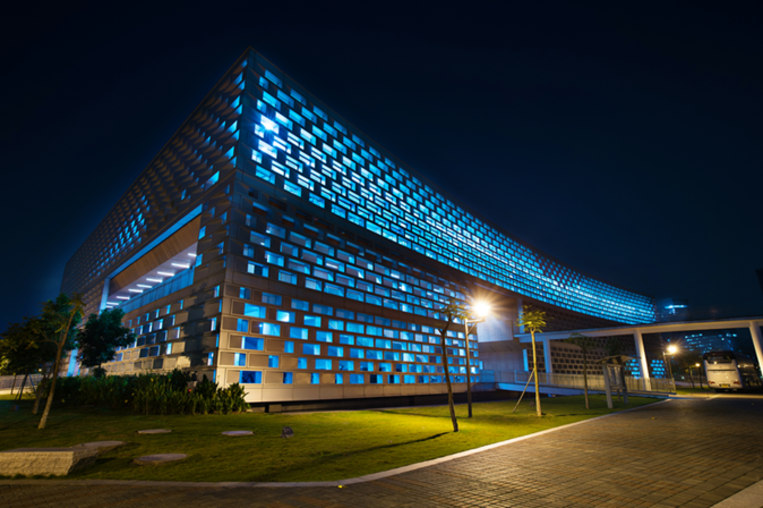
\includegraphics{figures/sustech.pdf}
		}
		%\includegraphics[scale=1.0]{figurefile}
		\caption{SUSTech Campus}
		\label{fig:campus}
	\end{figure}
\end{column}%
\hfill%
\begin{column}<0->{.65\textwidth}
	\begin{itemize}
		\item<1-> 短信息(SMS)成为现代通讯的重要组成部分
		\begin{itemize}
			\item<1-> 很多组织或网站使用短信息作为身份验证的辅助通道
		\end{itemize}
		\item<2-> 现代短消息的发送,在抵达终端之前不接触蜂窝网络
		\begin{itemize}
			\item<2-> 短信息(SMS)成为现代通讯的重要组成部分
		\end{itemize}
	\end{itemize}
\end{column}%
\end{columns}
\end{frame}
\subsection{主要工作}
\begin{frame}{主要工作}
完成这项工作需要如下步骤
\begin{itemize}
\item  对SMS数据进行迄今为止最大的挖掘分析
\item 评估良性短消息服务的安全态势
\item  刻画通过SMS网关进行的恶意行为
\end{itemize}
\end{frame}

 \begin{frame}
\frametitle{OTT服务}
\begin{figure}[!t]
	\centering
	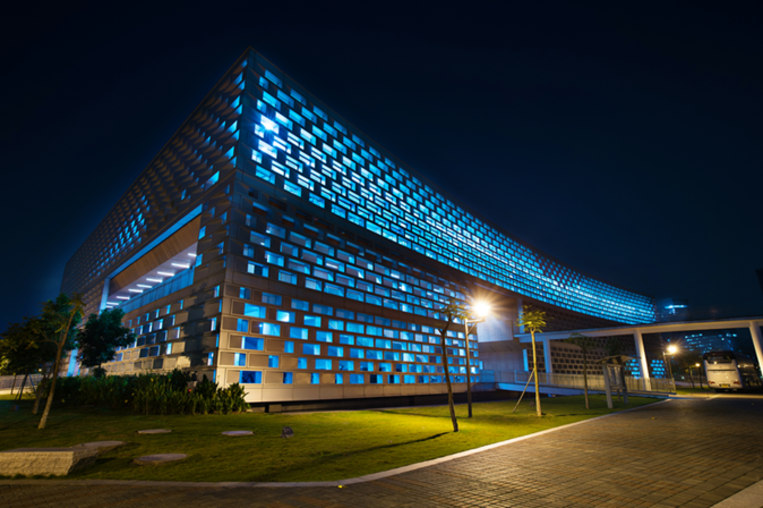
\includegraphics[width=2in]{figures/sustech.pdf}
	\caption{OTT服务}
	\label{figure3_OTT}
\end{figure}
\begin{center}
	OTT服务支持在数据网络上提供短信和语音等第三方服务。\\
	OTT可以使用云服务来存储和同步SMS到用户的其他设备。
\end{center}

\end{frame}

\begin{frame}{State of the art}
\begin{itemize}
\item Current anti-procrastination systems lack raw force
\begin{itemize}
\item Pomodoro, GTD, etc.
\end{itemize}
\item Raw force are often misused and in the wrong hands
\item People usually try to avoid punishment by telling lies
\end{itemize}
\end{frame}
% -----------------------------------------------------------------------------
\section{System Design}  %系统设计
\subsection{System Architecture}
\begin{frame}{System architecture}
\begin{columns}[T] % align columns
\begin{column}<0->{.48\textwidth}
\begin{figure}[thpb]
\centering
\resizebox{1\linewidth}{!}{
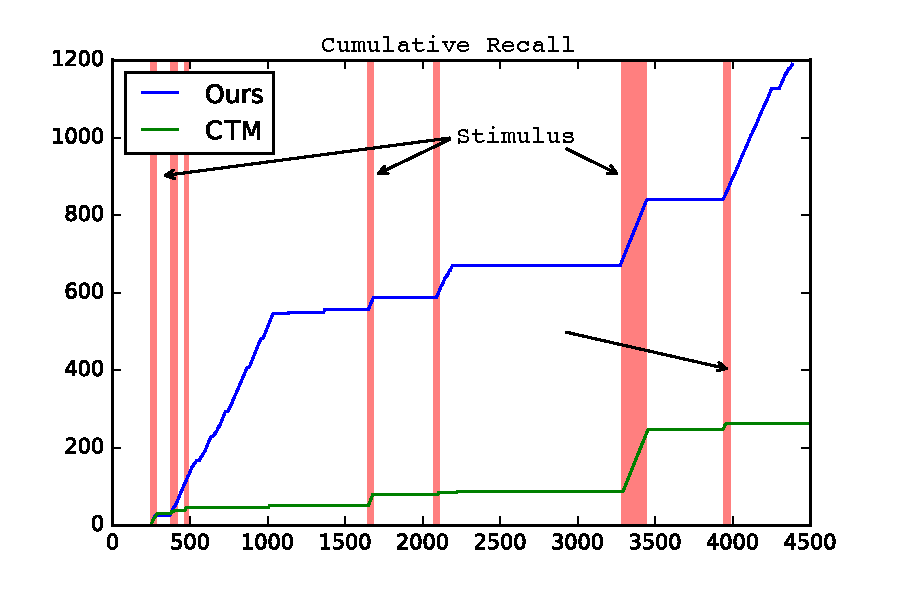
\includegraphics{figures/loss.pdf}
}
%\includegraphics[scale=1.0]{figurefile}
\caption{System components}
\label{fig:system}
\end{figure}
\end{column}%
\hfill%
\begin{column}<0->{.48\textwidth}
\begin{itemize}
\item Electric Chair: Punishment
\item Sensor: Detect behavior
\item Handcuffs: Raw confinement
\end{itemize}
\end{column}%
\end{columns}
\end{frame}
\begin{frame}{Tracking Results}
\begin{columns}[T] % align columns
\begin{column}<0->{.48\textwidth}
\begin{figure}[thpb]
\centering
\resizebox{\linewidth}{!}{
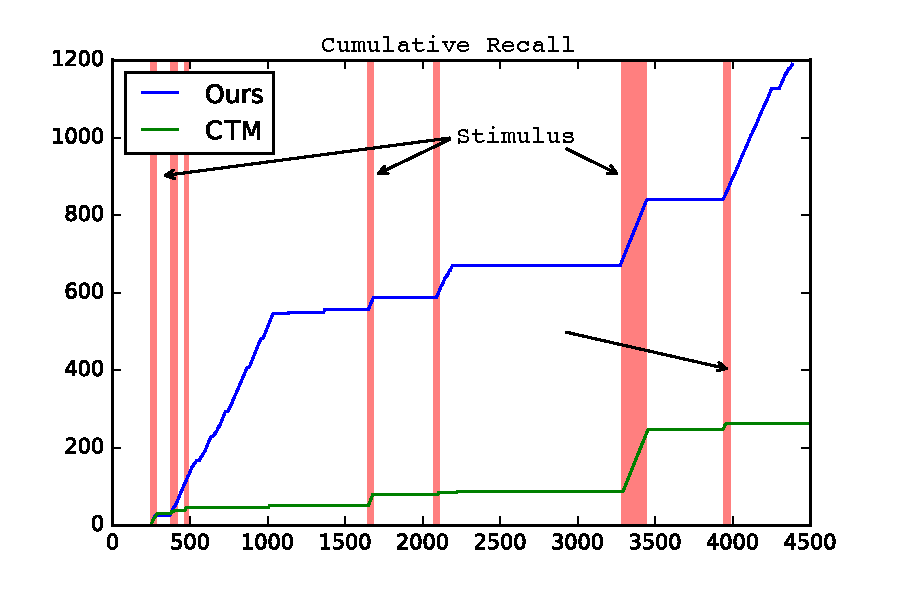
\includegraphics{figures/loss.pdf}
}
%\includegraphics[scale=1.0]{figurefile}
\caption{Effect of Electric Shock}
\label{fig:stimulus}
\end{figure}
\end{column}
\begin{column}<0->{.48\textwidth}
\begin{itemize}
\item Electric shock indeed improves the memory of subjects
\item This is a big loss for Big Brother
\end{itemize}
\end{column}
\end{columns}
\end{frame}
\subsection{Demo}  %成果展示
\begin{frame}{Demo}

\end{frame}
% -----------------------------------------------------------------------------
\section{Recap}

\subsection{Ongoing Study}
\begin{frame}{Recap}  %总结
In the paper:
\begin{itemize}
\item Proposed an electric-shock-based memory enhancement system that
\begin{itemize}
\item Uses handcuffs to confine user
\item Can maintain reliable performance in real-world conditions
\end{itemize}
\item Implemented such a system and proved that
\begin{itemize}
\item It really works\textsuperscript{TM}
\end{itemize}
\end{itemize}
\end{frame}

\subsection{研究方法与数据集特征}
\begin{frame}{研究方法与数据集特征}
\begin{columns}[T] % align columns
	\begin{column}<0->{.5\textwidth}
		\vspace*{1cm}
		\begin{itemize}
			\item 使用Scrapy框架爬取公共网关
		\end{itemize}
	
		\begin{itemize}
			\item 收集8个公共短信网关在14个月的数据
		\end{itemize}
	
		\begin{itemize}
			\item 共抓取386,327条数据
		\end{itemize}
    \end{column}%
\hfill%	
	\begin{column}<0->{.40\textwidth}
		\begin{table}
			\caption{公共网关及抓取的信息数}
			\label{table1:gateways}
			\centering
			\footnotesize
			\begin{tabular}{|c|c|}
				\hline
				\textbf{Site}           & \textbf{Messages}\\
				\hline
				receivesmsonline.net    &81313\\
				\hline
				receive-sms-online.info &69389\\
				\hline
				receive-sms-now.com     &63797\\
				\hline
				hs3x.com               &55499\\
				\hline
				receivesmsonline.com    &44640\\
				\hline
				receivefreesms.com      &37485\\
				\hline
				receive-sms-online.com  &27094\\
				\hline
				e-receivesms.com       &7107\\
				\hline
			\end{tabular}
		\end{table}
    \end{column}%
\end{columns}
\end{frame}

\begin{frame}
\frametitle{消息聚类分析}
\begin{block}{\textbf{基本思路}}
	\begin{itemize}
		\item 使用编辑距离矩阵将类似的消息归于一张连通图中。
		\item 使用固定值替换感兴趣的消息,如代码、email地址。
		\item 查找归一化距离小于阈值的消息,并确定聚类边界。
	\end{itemize}
\end{block}

\begin{block}{\textbf{实现步骤}}
	\begin{enumerate}
		\item 加载所有消息。
		\item 用固定的字符串替换数字、电子邮件和URL以预处理消息。
		\item 将预处理后的信息按字母排序。
		\item 通过使用编辑距离阈值(0.9)来确定聚类边界。
		\item 手动标记各个聚类,以确定服务提供者、消息类别等。
	\end{enumerate}
\end{block}
\end{frame}

\subsection{算法}
\begin{frame}{算法}
\begin{columns}[T] % align columns
   	\begin{column}<0->{.5\textwidth}
   	\begin{algorithm}[H]  
   		\caption{algorithm caption} %算法的名字
   		\hspace*{0.02in} {\bf Input:} %算法的输入, \hspace*{0.02in}用来控制位置,同时利用 \\ 进行换行
   		input parameters A, B, C\\
   		\hspace*{0.02in} {\bf Output:} %算法的结果输出
   		output result 
   		\begin{algorithmic}[1] %每行显示行号  
   		\State some description % \State 后写一般语句
   		\For{condition} % For 语句,需要和EndFor对应
   		\State ...
   		\If{condition} % If 语句,需要和EndIf对应
   		\Else
   		\EndIf
   		\EndFor
   		\While{condition} % While语句,需要和EndWhile对应
   		\EndWhile
   		\State \Return result	
   		\end{algorithmic}  
   	\end{algorithm}
   	\end{column}%
   \hfill%	
    \begin{column}<0->{.40\textwidth}
 
   	\end{column}%
   \end{columns}
\end{frame}

\begin{frame}[fragile]{代码}
\fontspec{Consolas}
\begin{lstlisting}
inline int gcd(int a, int b) { 
return b==0?a:gcd(b,a%b)
}
inline int lcm(int a, int b) {
return a/gcd(a,b)*b;
}
\end{lstlisting}
\end{frame}


\subsection{Future Work}
\begin{frame}{Future Work}  %将来可做的方向
\begin{itemize}
\item Get more people to try this
\item Benchmark the entire system in the wild
\item Profit!
\end{itemize}
\end{frame}

\begin{frame}{Thank you}
\begin{center}
\begin{minipage}{1\textwidth}
	\setbeamercolor{mybox}{fg=white, bg=black!50!blue}
 \begin{beamercolorbox}[wd=0.70\textwidth, rounded=true, shadow=true]{mybox}
\LARGE \centering Thank you for listening!  %结束语
\end{beamercolorbox}
 \end{minipage}
\end{center}
\end{frame}

\begin{frame}{Q\&A}
\begin{center}
	\begin{minipage}{1\textwidth}
		\setbeamercolor{mybox}{fg=white, bg=black!50!blue}
		\begin{beamercolorbox}[wd=0.70\textwidth, rounded=true, shadow=true]{mybox}
			\LARGE \centering  Questions?  %请求提问
		\end{beamercolorbox}
	\end{minipage}
\end{center}
\end{frame}

% -----------------------------------------------------------------------------
\end{document}
%文档结束